
\subsection{Quality tests to patterns and $PIV$ parameters}
\label{sec:qualitytests}
In the next tests we compare 3 types of patterns, over the beams, 
that we call $PA$, $PB$ and $PC$ like presented in 
Fig. \ref{fig:samplesabc}.

\subsubsection{Quality test-1: Displacement test}
The displacement test (test-1) shows the variation of $PCC$ between two analysis regions,
displaced a distance $d$, in a test object with a certain pattern in the surface. 
Thus, being specific,
the test-1 (presented in the Algorithm \ref{alg:displacementtest} of Section \ref{sec:algorithm})
shows the correlations obtained between two square analysis 
regions ($A_{i_0 j_0}$ and $A_{ij}$),
of $WSIZE$ pixels of side, separated by a distance $d=\sqrt{(i-i_0)^2+(j-j_0)^2}$ in pixels.
The initial analysis region is $A_{i_0 j_0}$, and it is chosen in the pixel position $(i_0,j_0)$, 
later this is compared with all others analysis 
regions $A_{ij}$, chosen in the pixel position $(i,j)$, $\forall~i,j \in Z^+|~ 0 \leq |i-i_0| < L$, $~ 0 \leq |j-j_0| < L$.
Thus, for purposes of this analysis we use the patterns $PA$, $PB$ and $PC$ in the side of beam, with
3 different values to $WSIZE$ ($16$, $32$ and $64$).
The next figures show the the result of ``displacement test'' from a pixel position $(i_0,j_0)$.


The Figs. \ref{fig:choosingA16}, \ref{fig:choosingB16} and \ref{fig:choosingC16}
represent the result of displacement test to $WSIZE=16$, 
in the patterns $PA$, $PB$ and $PC$ respectively.
It can be appreciated that in the center of each image exist a maximum of correlation
with value $\rho_0=1.0$, that correspond to the correlation of  $A_{i_0 j_0}$ and $A_{ij}$,
when $i=i_0$ and  $j=j_0$. 
The correlation $\rho_i$ between $A_{i_0 j_0}$ and $A_{ij}$ to $i\neq i_0$ and  $j\neq j_0$;
to the case of pattern $PA$ (Painted with spray) is medium in relation to $\rho_0$
with a maximum value $\rho_i$ of $0.5$, approximately, this condition is acceptable
because if is used a high value of match threshold, then It is 
guaranteed that the region $A_{i_0 j_0}$ only match with itself;
to the case of pattern $PB$ (Grid of dots) the correlation is high in relation to $\rho_0$
with a maximum value $\rho_i$ of $0.9$, approximately, this condition is 
very bad because it can bring false positives in the match of two analysis regions; Finally,
to the case of pattern $PC$ (Aleatory dots) the correlation is medium almost high in relation to $\rho_0$
with a maximum value $\rho_i$ of $0.65$, approximately, this condition is
slightly dangerous because if we use a very low match threshold we can have 
an identification error of the region $A_{i_0 j_0}$.
\begin{figure}[H]
  \centering
  \begin{subfigure}[b]{0.45\textwidth}
    \includegraphics[width=\textwidth]{image_plotA-16.eps}
    \vspace{2pt}
    \caption{Test of pattern $A$.}
    \label{fig:choosingA16}
  \end{subfigure}
  \begin{subfigure}[b]{0.45\textwidth}
    \includegraphics[width=\textwidth]{image_plotB-16.eps}
    \vspace{2pt}
    \caption{Test of pattern $B$.}
    \label{fig:choosingB16}
  \end{subfigure}
  \begin{subfigure}[b]{0.45\textwidth}
    \includegraphics[width=\textwidth]{image_plotC-16.eps}
    \vspace{2pt}
    \caption{Test of pattern $C$.}
    \label{fig:choosingC16}
  \end{subfigure}
  \caption{Displacement test to $WSIZE=16$.}
  \label{fig:choosingAll16}
\end{figure}


The Figs. \ref{fig:choosingA32}, \ref{fig:choosingB32} and \ref{fig:choosingC32}
represent the result of displacement test to $WSIZE=32$, 
in the patterns $PA$, $PB$ and $PC$ respectively. Similarly to the last case,
It can be appreciated that in the center of each image exist a maximum of correlation
with value $\rho_0=1.0$. Thus,
the correlation $\rho_i$ between $A_{i_0 j_0}$ and $A_{ij}$ to $i\neq i_0$ and  $j\neq j_0$;
to the case of pattern $PA$ (Painted with spray) is very low in relation to $\rho_0$
with a maximum value $\rho_i$ of $0.2$, approximately, 
so that the region $A_{i_0 j_0}$ only match with itself;
to the case of pattern $PB$ (Grid of dots) the correlation is medium in relation to $\rho_0$
with a maximum value $\rho_i$ of $0.8$, approximately, this condition is 
very bad because it can bring false positives in the match of two analysis regions; Finally,
to the case of pattern $PC$ (Aleatory dots) the correlation is very low in relation to $\rho_0$
with a maximum value $\rho_i$ of $0.4$, approximately, this condition is acceptable
because if is used a high value of match threshold, then It is 
guaranteed that the region $A_{i_0 j_0}$ only match with itself;
\begin{figure}[H]
  \centering
  \begin{subfigure}[b]{0.45\textwidth}
    \includegraphics[width=\textwidth]{image_plotA-32.eps}
    \vspace{2pt}
    \caption{Test of pattern $A$.}
    \label{fig:choosingA32}
  \end{subfigure}
  \begin{subfigure}[b]{0.45\textwidth}
    \includegraphics[width=\textwidth]{image_plotB-32.eps}
    \vspace{2pt}  
    \caption{Test of pattern $B$.}
    \label{fig:choosingB32}
  \end{subfigure}
  \begin{subfigure}[b]{0.45\textwidth}
    \includegraphics[width=\textwidth]{image_plotC-32.eps}
    \vspace{2pt}
    \caption{Test of pattern $C$.}
    \label{fig:choosingC32}
  \end{subfigure}
  \caption{Displacement test to $WSIZE=32$.}
  \label{fig:choosingAll32}
\end{figure}

The Figs. \ref{fig:choosingA64}, \ref{fig:choosingB64} and \ref{fig:choosingC64}
represent the result of displacement test to $WSIZE=64$, 
in the patterns $PA$, $PB$ and $PC$ respectively. Similarly to the last case,
It can be appreciated that in the center of each image exist a maximum of correlation
with value $\rho_0=1.0$. Thus,
the correlation $\rho_i$ between $A_{i_0 j_0}$ and $A_{ij}$ to $i\neq i_0$ and  $j\neq j_0$;
to the case of pattern $PA$ (Painted with spray) is low in relation to $\rho_0$
with a maximum value $\rho_i$ of $0.3$, approximately, 
so that the region $A_{i_0 j_0}$ only match with itself;
to the case of pattern $PB$ (Grid of dots) the correlation is medium in relation to $\rho_0$
with a maximum value $\rho_i$ of $0.8$, approximately, this condition is 
very bad because it can bring false positives in the match of two analysis regions; Finally,
to the case of pattern $PC$ (Aleatory dots) the correlation is very low in relation to $\rho_0$
with a maximum value $\rho_i$ of $0.2$, approximately, 
so that the region $A_{i_0 j_0}$ only match with itself;
\begin{figure}[H]
\centering
  \begin{subfigure}[b]{0.45\textwidth}
    \includegraphics[width=\textwidth]{image_plotA-64.eps}
    \vspace{2pt}
    \caption{Test of pattern $A$.}
    \label{fig:choosingA64}
  \end{subfigure}
  \begin{subfigure}[b]{0.45\textwidth}
    \includegraphics[width=\textwidth]{image_plotB-64.eps}
    \vspace{2pt}
    \caption{Test of pattern $B$.}
    \label{fig:choosingB64}
  \end{subfigure}
  \begin{subfigure}[b]{0.45\textwidth}
    \includegraphics[width=\textwidth]{image_plotC-64.eps}
    \vspace{2pt}
    \caption{Test of pattern $C$.}
    \label{fig:choosingC64}
  \end{subfigure}
  \caption{Displacement test to $WSIZE=64$.}
  \label{fig:choosingAll64}
\end{figure}

Finally, to a better understanding of the data in the Figs.
\ref{fig:choosingAll16}, \ref{fig:choosingAll32} and \ref{fig:choosingAll64},
they were create the Figs. 
\ref{fig:choosingt16}, \ref{fig:choosingt32} and \ref{fig:choosingt64},
 respectively.
Each new figure represents in a polar diagram around $(i_0,j_0)$, the lost of correlation
of the $3$ different patterns; so that the
distance $d$ in pixels represent a distance to position $(i_0,j_0)$; 
it is important to note in the figures that, if many pixel positions
represent the same distance, then only It is plotted the value with the highest correlation.
Thus, this new figures allow us to intuit, using a two-dimensional graphic,
how can exist false positives in the matching with regions neighboring to the origin.
\begin{figure}[H]
\centering
  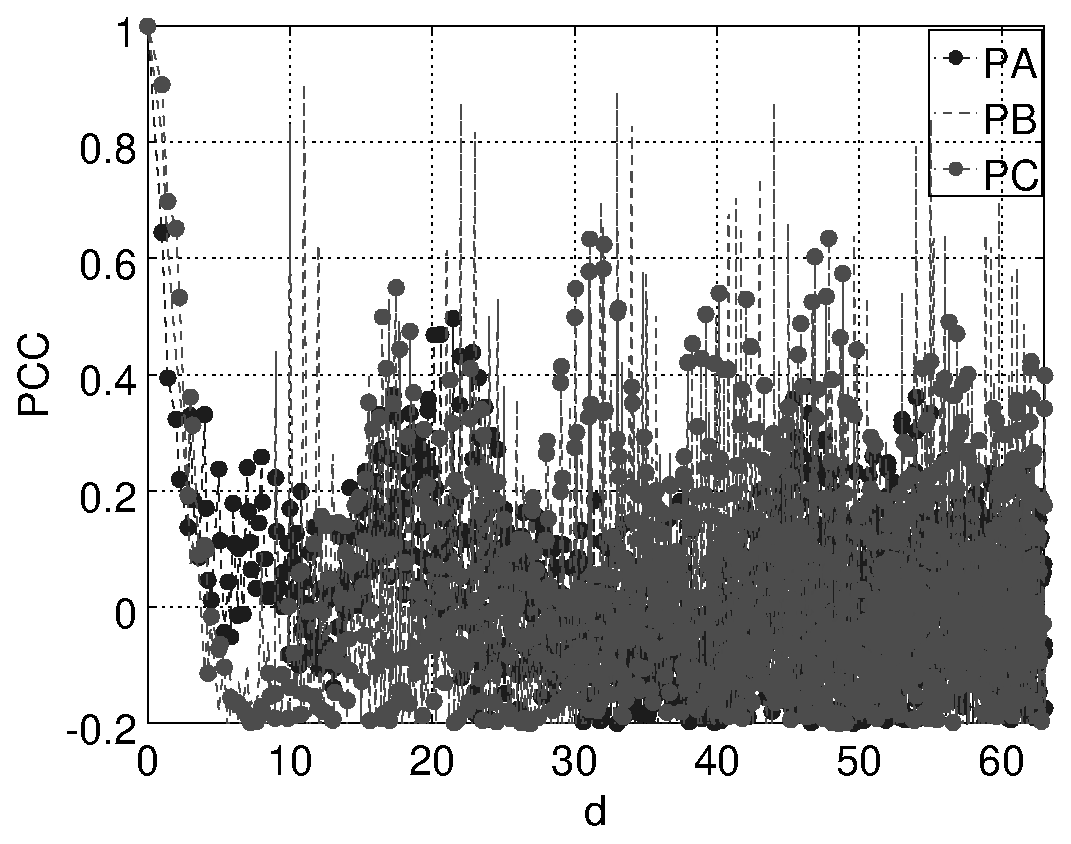
\includegraphics[width=.55\columnwidth]{image_plot-16.eps}
  \caption{Correlation of analysis regions in relation to the distance to $(i_0,j_0)$ to a $WSIZE=16$.}
  \label{fig:choosingt16}
\end{figure}
For example, in the Fig. \ref{fig:choosingt16} to the patterns $PA$, $PB$ and $PC$,
exist a high $PCC$ with analysis regions distant beyond 8 pixels, so that
It is very possible exist a false positive in the identification of a analysis 
region. The worst case is  obtained using the pattern $PB$, that reaches higher values
to $0.8$ in the correlation; the periodicity of $PCC$ value in this pattern
is a consequence of the periodicity of pattern.
\begin{figure}[H]
\centering
  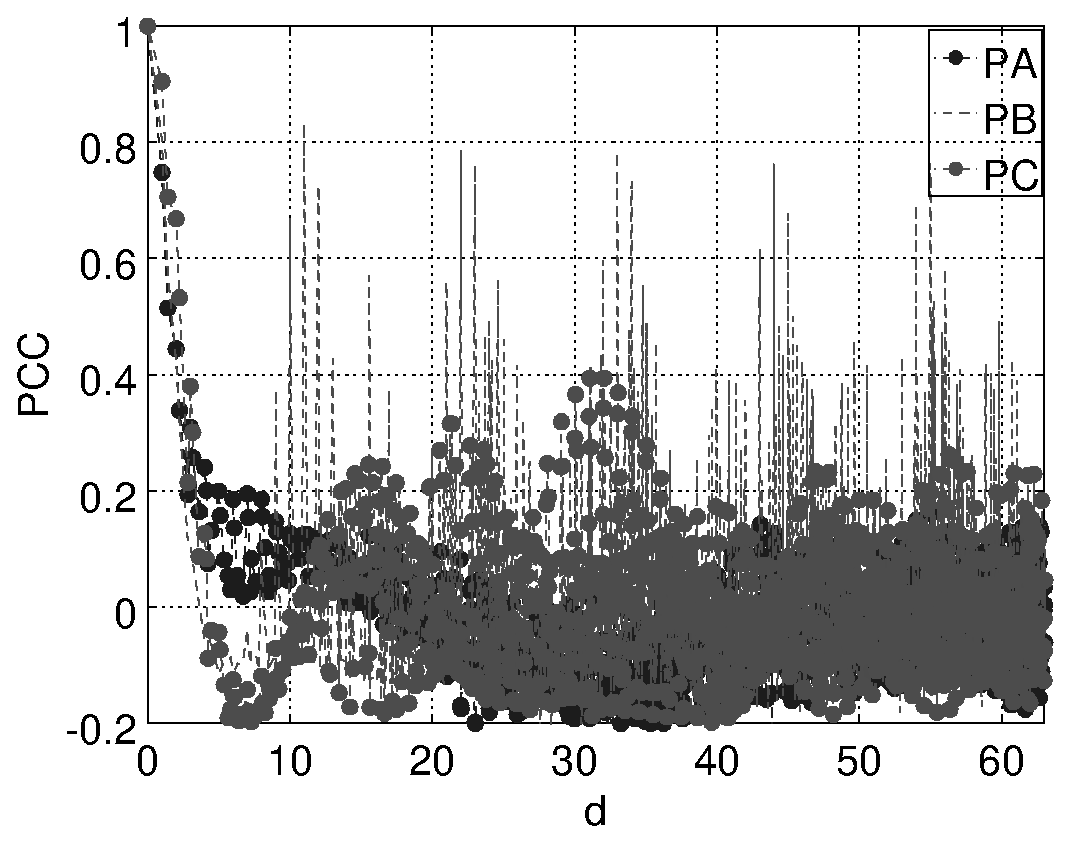
\includegraphics[width=.55\columnwidth]{image_plot-32.eps}
  \caption{Correlation of analysis regions in relation to the distance to $(i_0,j_0)$ to a $WSIZE=32$.}
  \label{fig:choosingt32}
\end{figure}
By other side, in the Fig. \ref{fig:choosingt32}, the $PCC$ value decays irregularly with 
distance in the patterns $PA$ and $PC$, as expected. But the pattern $PB$ still 
a high level of correlation with  peaks located with periodicity.
\begin{figure}[H]
\centering
  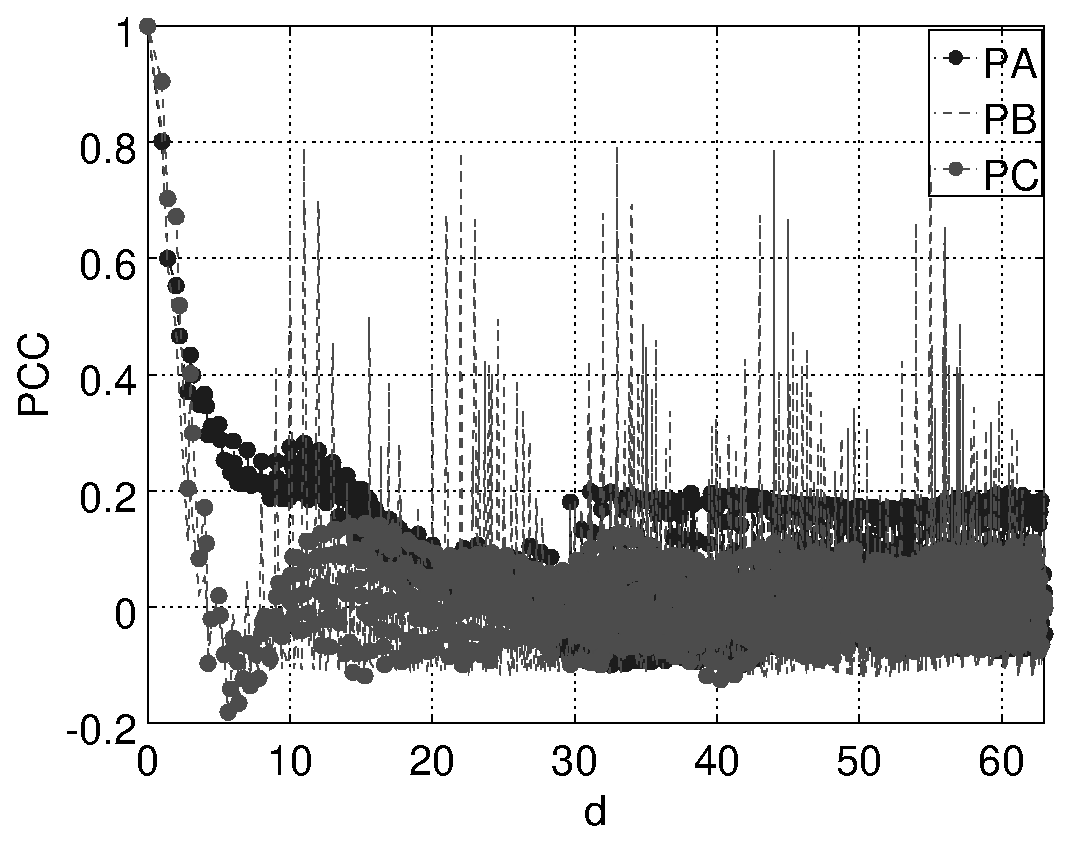
\includegraphics[width=.55\columnwidth]{image_plot-64.eps}
  \caption{Correlation of analysis regions in relation to the distance to $(i_0,j_0)$ to a $WSIZE=64$.}
  \label{fig:choosingt64}
\end{figure}
Finally, in the Fig. \ref{fig:choosingt64}, the $PCC$ value decays monotonously with 
distance in the patterns $PA$ and $PC$. The pattern $PB$ continues to have 
correlation problems.
